\documentclass[10pt]{article}

\usepackage{fancyhdr}
\usepackage[includeheadfoot,left=1in, right=1in, top=0.5in, bottom=0.5in]{geometry}
\usepackage{lastpage}
\usepackage{extramarks}
\usepackage[usenames,dvipsnames]{color}
\usepackage{graphicx}
\usepackage{listings}
%\usepackage{courier}
\usepackage{float}
\usepackage{url}
\usepackage{subfigure}
\usepackage{varwidth}
\usepackage{caption}
\usepackage{multirow}
\usepackage[pdfborder={0 0 0}]{hyperref}
\usepackage[compact,small]{titlesec}
\usepackage{microtype}
\usepackage{verbatim}
\usepackage{booktabs}
\usepackage{indentfirst}
\usepackage{pgffor}
\usepackage[table]{xcolor}
\usepackage{bytefield}
\usepackage{textcomp}
\usepackage{lipsum}

%\rowcolors{2}{gray!25}{white}

\parskip = 0.5\baselineskip
\setlength{\belowcaptionskip}{-\baselineskip}

\captionsetup{font=scriptsize}
\captionsetup{labelfont=bf}

\pagestyle{fancy}
\rhead{Max Thrun}
\lhead{8-Bit Softcore CPU}
\rfoot{Page\ \thepage\ of \protect\pageref{LastPage}}
\cfoot{}
\renewcommand\headrulewidth{0.4pt}
\renewcommand\footrulewidth{0.4pt}

% make verbatim text small
\makeatletter
\g@addto@macro\@verbatim\tiny
\makeatother

\setlength\parindent{0pt} % Removes all indentation from paragraphs

\definecolor{sh_comment}{rgb}{0.12, 0.38, 0.18 } %adjusted, in Eclipse: {0.25, 0.42, 0.30 } = #3F6A4D
\definecolor{sh_keyword}{rgb}{0.37, 0.08, 0.25}  % #5F1441
\definecolor{sh_string}{rgb}{0.06, 0.10, 0.98} % #101AF9

\lstset{
    language={[x86masm]Assembler},
    xleftmargin=.25in,
    xrightmargin=.25in,
    numbers=left,
    numberstyle=\tiny,
    frame=tb,
    showstringspaces=false,
    captionpos=b,
    stringstyle=\color{sh_string},
    keywordstyle = \color{sh_keyword}\bfseries,
    commentstyle=\color{sh_comment}\itshape,
    basicstyle=\footnotesize\sffamily,
    morekeywords={.define,stl,ld,brz,ldl},
    %numbersep=-5pt,
    belowskip=\baselineskip,
    aboveskip=\baselineskip
}

\let\oldtabular\tabular
\renewcommand{\tabular}{\footnotesize\oldtabular}

\newcommand{\placementimage}[2]{
    \begin{figure}[H]
        \centering
        \includegraphics[width=\linewidth, height=4in, keepaspectratio]{#1}
        \caption{#2}
    \end{figure}
}

\newcommand{\specialcell}[2][c]{\textbf{\begin{tabular}[#1]{@{}c@{}}#2\end{tabular}}}

\title{
    \vspace{0.5in}
    \textmd{\textbf{8-Bit Softcore CPU}}\\
    \vspace{2in}
    \textmd{\textbf{Submitted as the Capstone Project for\\the Master of Engineering Degree}}\\
    \vfill
}
\author{\textbf{Max Thrun}}

\begin{document}
\clearpage\maketitle
\thispagestyle{empty}
\newpage
\section{Abstract}

The purpose of this project is to create a custom 8-bit softcore computer
processing unit (CPU) which can ultimately be used and expanded on for both
educational and practical purposes. This project explores the design and
implementation of a complete system on chip (SoC) in the hardware description
language Verilog and realized on a field programmable gate array (FPGA). A
simple assembler and program loader, written in Python, are also developed in
order to form a complete development package. With these components we are able
to compile programs written in our custom assembly language and run them on our
custom CPU in a FPGA development board.

\section{Introduction}

The understanding, design, and implementation of a computer processing unit is
something that is often challenging for most people when they are first
studying the field. There are seemingly infinite resources on the subject but
there are very few that provide an easily digestible top to bottom example
going from the compiler down to the hardware.

When I personally started studying the topic of CPUs I had a strong urge to
implement my own and be able to compile and run small programs on it, which is a
sentiment I feel is common amongst people first getting interested in the
topic.  Like many, I have found that I often learn best by example and I was
frustrated with the lack of easy to understand example projects out
there. It was not until I came across the Your First CPU! \cite{yfcpu} blog
posts, which provided a simple concrete example of implementing a CPU, that
things really clicked. The Your First CPU!  blog posts were good at helping me
get an understanding of a CPU on the hardware level but it left a lot to be
desired on the software end as it provided fairly complex Flex and Bison
\cite{flex} scripts to parse and assemble programs. While these tools are
popular and extremely powerful I felt that they were over complicated for what
I wanted to achieve at the time which was to just simply compile a small
program and run it on my custom CPU.

There are numerous other example projects out there of CPUs but most that I
have come across in the past were either too complex, incomplete, or just
implemented in a way that I personally found confusing.  With this project I
try to bridge some of these gaps by providing a small, simple, working example
of a CPU as well as providing a basic assembler and a tool to load and run
programs.

\newpage
\section{Implementation}

    \subsection{Design Overview}

    The main goal of this project is to show an example of a working CPU. While
    this can be achieved purely through simulation it is much more satisfying
    to see a physical implementation running on a development board which can
    provide various inputs and outputs (IO).  For my implementation I chose to
    use an Altera DE-1 development board which has a Cyclone II FPGA and a
    plethora of various IO such as LEDs, switches, 7 segment displays, as well
    as more complex peripherals such as audio.

    In order to communicate with these peripherals we need additional
    components besides the CPU. Firstly, we need random access memory (RAM)
    which we will use to store our program and which the program will use to
    store information while it is running. The Cyclone II, like most modern
    FPGAs, has internal RAM which we can use for this purpose.  Secondly, we
    need some general purpose input and output (referred to as GPI and GPO in
    this project) modules in order to interface with peripherals such as LEDs
    and switches. Additionally, we would like to have some way of performing
    timed events, such as flashing the LEDs a certain rate. A 32-bit timer
    module has been implemented to achieve this. When the CPU needs to read or
    write data we need module which can determine if the CPU is trying to talk
    to RAM or a peripheral. This module is called a memory mapper as it maps
    different memory locations as seen by the CPU to various other components
    throughout the system. Finally, we need a way to load the programs into the
    system which is achieved by a serial bootloader.

    A system block diagram which illustrates the connection between the DE-1
    peripherals and the various components in the design is shown below.

    \begin{figure}[H]
        \centering
        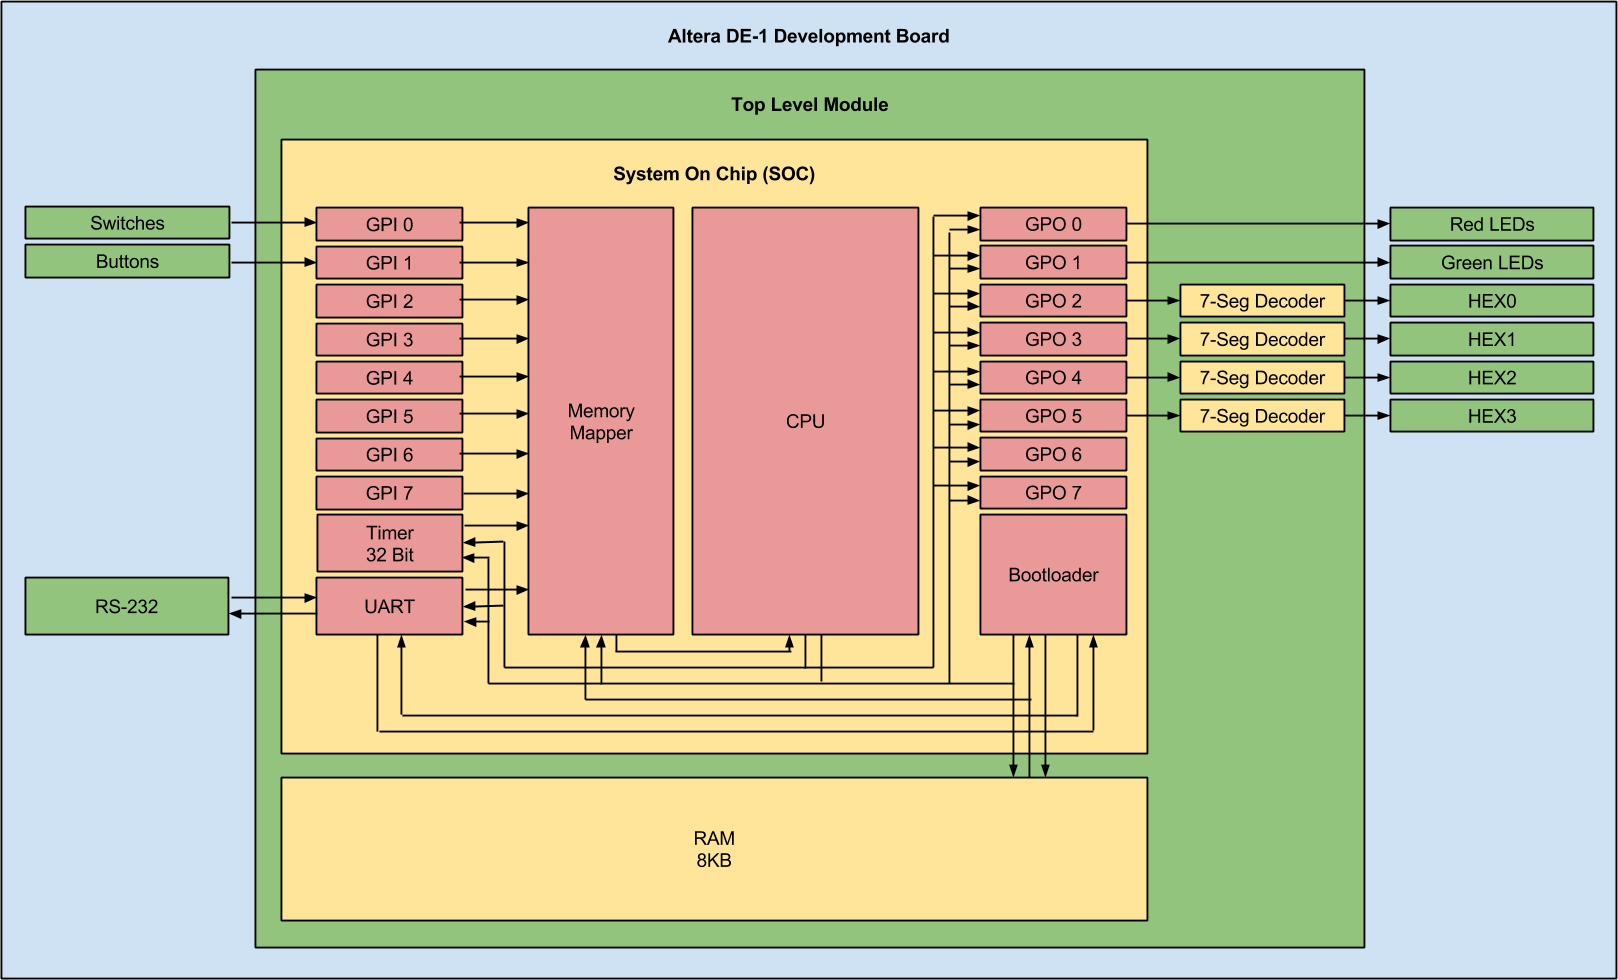
\includegraphics[width=\linewidth]{./block_diagram.png}
        \caption{System Block Diagram}
    \end{figure}



    \subsection{CPU}

        \begin{figure}[H]
            \centering
            \begin{minipage}[t]{.7\textwidth}
                \vspace{0pt}
                The CPU for this project is non-piplined and each instruction
                takes 7 clock cycles to complete.  Additionally, I have chosen
                to go with a Von Neumann style architecture \cite{von} where
                the data and instructions are both stored in the same memory
                and accessed by a single bus. The reason for this over a
                Harvard style architecture \cite{harvard} is that it is
                slightly simpler to implement and also allows us to more easily
                achieve cool tricks such as having a program modify its own
                code \cite{modify}. One of the down sides of using a Von
                Neumann architecture is that you cannot access the instruction
                and data memory at the same time. This means that you would
                typically need a whole extra cycle just to fetch or store data.
                To avoid this I am actually clocking the CPU on the opposite
                edge of the clock relative to the rest of the system.  This
                means that the CPU steps on the positive edge and the memory
                responds on the negative edge which allows the data to be ready
                by the next CPU cycle. Doing this saves us up to 2 clock cycles
                per instruction.
            \end{minipage}%
            \begin{minipage}[t]{.3\textwidth}
                \vspace{0pt}
                \centering
                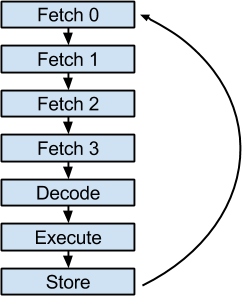
\includegraphics[width=0.5\linewidth]{./instruction_cycle.png}
                \caption{CPU Instruction Cycle}
            \end{minipage}
        \end{figure}

        Each instruction is 4 bytes long which requires 4 fetch stages to form
        the complete instruction word as our RAM only accesses single bytes at
        a time.  Typically, the next stage would be to decode the instruction
        being that in some instruction sets the operands might cross byte
        boundaries and you need to wait until you have fetched all the bytes
        before you can decode the instruction. To simplify things, in our CPU
        the opcode and each operand get their own separate byte with the
        exception of memory addresses which require two bytes.  The side effect
        of this is that each operand can address up to 256 registers which in
        practice is unusual (a typical CPU might only have a couple dozen
        registers at most). We will consider this huge register file a feature
        as it actually makes writing a high level language compiler
        significantly easier as you do not need to worry about high pressure
        register allocation.  Since we do not actually have to decode the
        instruction the decode stage is used to increment the program counter
        and switch the memory address that the CPU is looking at to the address
        of the data specified by the instruction.

        \vspace{\baselineskip}
        The table below summarizes the 22 instructions that are currently
        implemented.

        \begin{table}[H]
            \resizebox{\textwidth}{!}{%
            \centering
            \begin{tabular}{lllc}
                \toprule
                \textbf{Mnemonic} & \textbf{Operands} & \textbf{Description} & \specialcell{32-Bit Instruction Word\\MSb \hspace{1.75in} LSb}\\
                \midrule
                HALT &                 & Stop program execution                                         & \texttt{00000000 -------- -------- --------} \\
                LD   & \texttt{d,m} & Load value at address \texttt{m} into register \texttt{d}         & \texttt{00000001 dddddddd mmmmmmmm mmmmmmmm} \\
                ST   & \texttt{s,m} & Store register \texttt{s} into memory address \texttt{m}          & \texttt{00000010 ssssssss mmmmmmmm mmmmmmmm} \\
                STL  & \texttt{l,m} & Store literal \texttt{l} into memory address \texttt{m}            & \texttt{00000011 llllllll mmmmmmmm mmmmmmmm} \\
                LDL  & \texttt{d,l}    & Load literal \texttt{l} into register \texttt{d}               & \texttt{00000100 dddddddd aaaaaaaa --------} \\
                MOV  & \texttt{d,s}    & Move register \texttt{s} into register \texttt{d}              & \texttt{00000101 dddddddd aaaaaaaa --------} \\
                ADD  & \texttt{d,a,b}  & \texttt{d = a + b}                                             & \texttt{00000110 dddddddd aaaaaaaa bbbbbbbb} \\
                SUB  & \texttt{d,a,b}  & \texttt{d = a - b}                                             & \texttt{00000111 dddddddd aaaaaaaa bbbbbbbb} \\
                AND  & \texttt{d,a,b}  & \texttt{d = a \& b}                                            & \texttt{00001000 dddddddd aaaaaaaa bbbbbbbb} \\
                OR   & \texttt{d,a,b}  & \texttt{d = a | b}                                             & \texttt{00001001 dddddddd aaaaaaaa bbbbbbbb} \\
                XOR  & \texttt{d,a,b}  & \texttt{d = a $\oplus$ b}                                      & \texttt{00001010 dddddddd aaaaaaaa bbbbbbbb} \\
                SFL  & \texttt{d,a,b}  & \texttt{d = a << b}                                            & \texttt{00001011 dddddddd aaaaaaaa bbbbbbbb} \\
                SFR  & \texttt{d,a,b}  & \texttt{d = a << b}                                            & \texttt{00001100 dddddddd aaaaaaaa bbbbbbbb} \\
                INC  & \texttt{d,a,b}  & \texttt{d = a + 1}                                             & \texttt{00001101 dddddddd aaaaaaaa bbbbbbbb} \\
                DEC  & \texttt{d,a,b}  & \texttt{d = a - 1}                                             & \texttt{00001110 dddddddd aaaaaaaa bbbbbbbb} \\
                EQL  & \texttt{d,a,b}  & \texttt{d = a == b}                                            & \texttt{00001111 dddddddd aaaaaaaa bbbbbbbb} \\
                GTH  & \texttt{d,a,b}  & \texttt{d = a > b}                                             & \texttt{00010000 dddddddd aaaaaaaa bbbbbbbb} \\
                LTH  & \texttt{d,a,b}  & \texttt{d = a < b}                                             & \texttt{00010001 dddddddd aaaaaaaa bbbbbbbb} \\
                INV  & \texttt{d,a}    & \texttt{d = \texttildelow a}                                   & \texttt{00010010 dddddddd aaaaaaaa --------} \\
                BRZ  & \texttt{a,m} & Branch to \texttt{m} if register \texttt{a} is zero               & \texttt{00010011 aaaaaaaa mmmmmmmm mmmmmmmm} \\
                BRNZ & \texttt{a,m} & Branch to \texttt{m} if register \texttt{a} is not zero           & \texttt{00010100 aaaaaaaa mmmmmmmm mmmmmmmm} \\
                JMP  & \texttt{m}   & Jump to address \texttt{m}                                        & \texttt{00010101 mmmmmmmm mmmmmmmm --------} \\
                \bottomrule
        \end{tabular}}
            \caption{Instruction Set Description \& Encoding}
        \end{table}

    \subsection{Memory Mapping}

        \newcommand{\memsection}[4]{
            \bytefieldsetup{bitheight=#3\baselineskip}  % define the height of the memsection
            \bitbox[]{8}{
                \texttt{0x\uppercase{#1}}    % print end address
                \\ \vspace{#3\baselineskip} \vspace{-2\baselineskip} \vspace{-#3pt} % do some spacing
                \texttt{0x\uppercase{#2}} % print start address
            }
            \bitbox{16}{#4} % print box with caption
        }

        \newcommand{\memsectionone}[4]{
            \bytefieldsetup{bitheight=#3\baselineskip}  % define the height of the memsection
            \bitbox[]{8}{
                \texttt{0x\uppercase{#1}}    % print end address
                %\\ \vspace{#3\baselineskip} \vspace{-2\baselineskip} \vspace{-#3pt} % do some spacing
                %\texttt{0x\uppercase{#2}} % print start address
            }
            \bitbox{16}{#4} % print box with caption
        }

        \begin{figure}[H]
            \centering
            \begin{minipage}[t]{.5\textwidth}
                \vspace{0pt}
                All input, outputs, and internal peripherals such as the 32-bit
                timer and the UART are accessed and controlled via memory
                accesses in a scheme called memory-mapped IO \cite{io}. In this
                scheme each peripheral is assigned a memory address and then
                watches for this address on the memory bus. When the CPU writes
                to this address it stores the data to its own internal
                registers. When the CPU is doing a read we need a single entity
                in charge of figuring out which peripherals data to give to the
                CPU. This entity is called the memory mapper and it has a list
                of the memory addresses of all the peripherals. All the
                peripherals feed their outputs into the memory mapper.  The
                memory mapper then looks at the address that the CPU wants and
                feeds it the corresponding peripherals data. If the requested
                address does not belong to any peripheral the memory mapper
                selects the RAM as the CPU input.

                \vspace{\baselineskip}
                One downside of this approach is that we are wasting RAM. When
                the CPU writes to the memory address belonging to a peripheral
                that data also gets written into RAM but when the CPU reads
                back the memory at that address the memory mapper will direct
                the peripherals output to the CPU, not the RAMs output. In our
                case we have only a handful of memory mapped peripherals and
                lots of RAM so it is not a huge issue.
            \end{minipage}%
            \begin{minipage}[t]{.5\textwidth}
                \vspace{0pt}
                \centering
                \begin{bytefield}{24}
                    \memsection{FFFF}{0020}{15}{Program Space}\\
                    \memsection{0019}{0013}{2}{Reserved}\\
                    \memsectionone{0012}{0012}{1}{UART Control / Status}\\
                    \memsectionone{0011}{0011}{1}{UART TX Data}\\
                    \memsectionone{0010}{0010}{1}{UART RX Data}\\
                    \memsection{000F}{0008}{2}{General Purpose Outputs}\\
                    \memsection{0007}{0000}{2}{General Purpose Inputs}\\
                \end{bytefield}
                \caption{SoC Memory Map}
            \end{minipage}
        \end{figure}

        The diagram to the right shows the memory map of our address space.
        There are 8 GPI peripherals and 8 GPO peripheral and each one takes 1
        byte.  The UART uses 3 bytes, 2 for data in and out and a third one for
        status and control.  Addresses \texttt{0x0013} through \texttt{0x0019}
        are reserved for future peripherals that might be added. The program
        space starts at \texttt{0x0020} and extends all the way to
        \texttt{0xFFFF} which gives the program about 65KB of usable space (not
        accounting for the size of the program itself). Note that this is the
        maximum amount of memory that the CPU is capable of addressing, it does
        not mean that amount of RAM will actually be available. The amount of
        RAM in FPGAs varies so the size of the RAM is configurable at build
        time by setting the \texttt{RAM\_ADDR\_BITS} define in the
        \texttt{constants.v} file. In my case, I can only fit about 8KB of RAM
        in the Cyclone II that is on my development board. Most actual
        production SoCs contain internal RAM but since I am targeting FPGAs,
        which might not have a lot of internal RAM, I did not want to make
        internal RAM a hard requirement so I brought out the RAM interface.
        This makes it easy to use re-use the SoC module with external RAMs,
        such as the SRAM that is on my DE-1 development board.

    \subsection{Bootloader}

        \begin{figure}[H]
            \centering
            \begin{minipage}[t]{.6\textwidth}
                \vspace{0pt}
                One of the bigger challenges of running our system on an FPGA
                is loading the program into RAM.  Under simulation it is as easy
                as using the \texttt{\$readmemb("filename")} function but it is
                not as straight forward when targeting a physical device. It is
                possible to bake the program in with the FPGA bitstream using a
                memory initialization file \cite{mif} but this would require us
                to resynthesize and flash the FPGA every time we wanted to run
                a new program.

                \vspace{\baselineskip}
                Another obvious solution would be to store the program on an SD
                card and write a hardware state machine to read it. While this
                initially seems like an attractive solution due to the ubiquity
                of SD cards it has three major drawbacks: interfacing with an
                SD card is not simple, not all FPGA development boards have an
                SD card slot, and every time you want to update the program you
                have to remove the SD card, put it in your computer, change the
                program, take it out, put it back in the dev board, and reset
                the FPGA.  For rapid development, which is what we want to do,
                this process is unacceptable.

                \vspace{\baselineskip}
                Yet another solution is to load our program via a serial port.
                All FPGAs are capable of implementing a UART and getting a USB
                to UART adaptor is cheap and easy. Also, with this method we
                can simply press a button on the development board to put the
                system into `boot mode' and then run a little script on the
                computer to send the program over.  The only disadvantage of
                this method is that the program is volatile, if we power cycle
                the board we have to resend the program. Since the goals of
                this project do not involve embedding our FPGA into a system
                that needs to be able to survive power cycles the UART solution
                is great.
            \end{minipage}%
            \begin{minipage}[t]{.4\textwidth}
                \vspace{0pt}
                \centering
                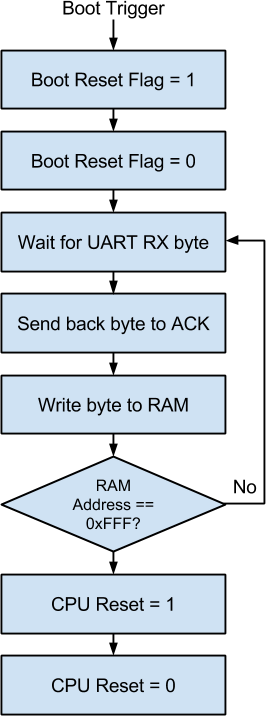
\includegraphics[width=0.65\linewidth]{./bootloader.png}
                \caption{Bootloader State Machine}
            \end{minipage}
        \end{figure}

        The UART bootloader needs to be able to do 2 main things: receive and
        write a program to RAM, and reset the CPU after it is done. The state
        diagram shown above illustrates this process. The state machine sits in
        an idle state until a boot trigger event, which I have mapped to a
        button on my development board. It then drops through two states which
        pulse the boot reset flag. This flag is used to reset the UART to clear
        any status flags that may be set. The bootloader also asserts a signal
        to indicate that it is in boot mode. This switches the RAMs address and
        data lines from the CPU to the bootloader. The bootloader then
        continuously reads bytes from the UART and loads them into RAM,
        incrementing the RAM address after each byte, until it reaches the top
        of the RAM. The disadvantage of this method is that we have to send the
        full RAM contents, even if it is mostly zeros. This is significantly
        slower than just sending the RAM contents that the program actually
        occupies.  A possible solution to this might be to run length encode
        the data but with small RAM sizes (like the one in our system) it only
        takes a few seconds to load so the effort of speeding it up is probably
        not worth it. Once the bootloader has determined that it has received
        all the bytes it puts the CPU in reset and de-asserts the boot mode
        flag. It then de-asserts the CPU reset line and execution begins. It is
        important to have the CPU in reset before de-asserting the boot mode
        flag as once the flag is de-asserted the CPU has control over the RAM.
        Since the contents of RAM were unknown and changing during boot the CPU
        could be executing anywhere. We don't want to give control of the RAM
        back to the CPU until we reset it.


    \newpage
    \subsection{Assembler}

    To construct a program that can run on our CPU we simply need to lookup the
    binary encoding of the instruction that we want to use. While it is
    certainly possible to assemble a program by hand it is much less tedious to
    have an assembler do it for you. I have created a simple assembler
    (\texttt{./tools/asm.py}) which supports some of the typical features one
    would expect from an assembler.

    The assembler reads the input \texttt{.asm} file line by line and first
    strips the line of comments and forces it to upper case. It then figures
    out if the line is a directive (like \texttt{.define}), an instruction, or
    a label. If it is an instruction it forms the 4 byte instruction word
    (using the OP code that it automatically parses out of the Verilog
    \texttt{constants.v} file) and adds those bytes to an array. If it comes
    across a label it records the name of the label and what byte location it
    is at. When it comes across a jump it records what the destination label is
    and then fills in zeros for the address since it might not know what the
    address of the label is yet (if it wants to jump forward in the program we
    do not yet know the address of that label).  After all instruction bytes
    have been added to the array it goes back through all the jumps, looks up
    the position of the label it wants to jump to, and fills out the address of
    the jump instruction. It then writes all the bytes out to two files: one
    file which is a raw binary file that we will load into the FPGA (called a
    ROM), and another which is an ASCII file formatted in a way that can be
    read in by the Verilog simulator.

    Other features such as aliases, the equivalent to \texttt{\#define} in C,
    are supported through the \texttt{.define} directive and comments are fully
    supported as well. The assembler also parses the \texttt{constants.v} file
    to figure out the memory location of all the memory mapped peripherals and
    automatically adds an alias for them. This is nice since when you add a new
    peripheral you only have to update the Verilog file and the assembler
    automatically will account for it. The whole assembler is only about 150
    lines of code, most of which is just putting the operands in the correct
    byte order for each instruction.

    An example program which increments the value shown on the  LEDs every time
    the timer goes off is shown below.

    \lstinputlisting[caption=Count up on the LEDs]{../tools/count.asm}


\newpage
\section{Results}

    The results of this project are best conveyed through video. The following
    videos show the CPU running four different test programs on the DE-1
    development board.

    \begin{table}[H]
        \centering
        \begin{tabular}{lll}
            \toprule
            \textbf{Test Program} & \textbf{Description} & \textbf{Video Link} \\
            \midrule
            \texttt{shift.asm}      & Shifts a single LED down both sets of LEDS     & \url{http://youtu.be/aNCSzHn3NVQ} \\
            \texttt{count.asm}      & Counts up in binary on the LEDs                & \url{http://youtu.be/9p6P2v8b_BA} \\
            \texttt{seg\_count.asm} & Counts up in base 10 on the 7-segment displays & \url{http://youtu.be/zjMZnJXbdMo} \\
            \texttt{blink\_1hz.asm} & Blinks the green LEDs at 1hz                   & \url{http://youtu.be/qbEIPBlEjM4} \\
            \bottomrule
        \end{tabular}
    \end{table}

    We can see from the videos above that the CPU and supporting components all
    seem to be working as expected. While these small test programs are no
    where near that complexity of what a typical application might be like it
    at least proves that the system is working at a fundamental level and that
    all of our development tools are working correctly. With just 2 lines of
    Verilog and 4 lines of Python we can add additional instructions to the CPU
    and start exploring more complex topics and designs in the future. Given
    the ease in which we can modify and extend this project I believe we have
    achieved the original goal of building a complete example system from the
    CPU all the way to the compiler.

\section{Discussion}

    I believe the efficacy of my implementation is strong given the overall
    success of the project. The original goal was to produce a small and simple
    example CPU and compiler that can be used primarily as a learning platform.
    While its effectiveness in conveying knowledge is yet to be determined the
    project is completely functional from a technical aspect. I believe I was
    able to keep it relatively simple while still achieving interesting
    features such as the 32-bit timer and serial bootloader.

    There are a few things I felt I have learned from this project. From a
    technical perspective I formed an appreciation for how much work goes into
    the details of CPU and system architecture design. Things that appear to be
    simple, like figuring out the instruction set architecture, can actually be
    fairly difficult when you sit down and try to figure out the best way to do
    it.  Fortunately with my project I was able to take a simpler approach for
    some of these problems as the whole goal of this project was simplicity. On a
    \emph{slightly} less technical level I feel that I improved my overall
    ability to gage the complexity of projects of this nature and improved my
    approach to solving them.

    There are literally an infinite number of things that could be improved or
    added to this project. Anything from new CPU instructions, to peripherals,
    to compiler directives. A few features that I feel would be interesting to
    add are peripherals for I2C and SPI (common communication protocols), a
    small VGA peripheral that exposes one side of a dual port ram to the CPU,
    an example program that can read and write to an SD card (which uses SPI),
    addition math instructions such as divide and multiply, compiler directives
    to include arbitrary data in the ROM such as text and images, a directive
    to specify where certain blocks of instructions are loaded into RAM, basic
    interrupt support... the possibilities for expansion are endless.

\vfill
All project files can be viewed here:\\
\url{https://github.com/bear24rw/EECE9060.git}

Or as a \texttt{.zip} download:\\
\url{https://github.com/bear24rw/EECE9060/archive/master.zip}


\newpage
\begin{thebibliography}{9}

    % \cite{gg}
    %\bibitem{gg} \url{http://mo5.com/musee-machines-gamegear.html}
    \bibitem{yfcpu} \url{http://colinmackenzie.net/index.php?option=com_content&view=article&id=11:your-first-cpu&catid=8:rotator&Itemid=7}
    \bibitem{flex} \url{http://aquamentus.com/flex_bison.html}
    \bibitem{cycle} \url{http://en.wikipedia.org/wiki/Instruction_cycle}
    \bibitem{von} \url{http://en.wikipedia.org/wiki/Von_Neumann_architecture}
    \bibitem{modify} \url{http://en.wikipedia.org/wiki/Self-modifying_code}
    \bibitem{harvard} \url{http://en.wikipedia.org/wiki/Harvard_architecture}
    \bibitem{io} \url{http://en.wikipedia.org/wiki/Memory-mapped_I/O}
    \bibitem{mif} \url{http://quartushelp.altera.com/13.0/mergedProjects/reference/glossary/def_mif.htm}
\end{thebibliography}

\newpage
\section*{Example Programs}
        \lstinputlisting[basicstyle=\tiny,caption=count.asm]{../tools/count.asm}
        \lstinputlisting[basicstyle=\tiny,caption=shift.asm]{../tools/shift.asm}
        \lstinputlisting[basicstyle=\tiny,caption=blink\_1hz.asm]{../tools/blink_1hz.asm}
        \lstinputlisting[basicstyle=\tiny,caption=seg\_count.asm]{../tools/seg_count.asm}

\newpage
\section*{Python Code}
        \lstinputlisting[basicstyle=\tiny,caption=asm.py,language=Python]{../tools/asm.py}
        \lstinputlisting[basicstyle=\tiny,caption=send\_rom.py,language=Python]{../tools/send_rom.py}

\newpage
\section*{Verilog Code}
            \lstinputlisting[basicstyle=\tiny,caption=top.v,language=Verilog]{../rtl/top.v}
\newpage    \lstinputlisting[basicstyle=\tiny,caption=soc.v,language=Verilog]{../rtl/soc.v}
            \lstinputlisting[basicstyle=\tiny,caption=ram.v,language=Verilog]{../rtl/ram.v}
\newpage    \lstinputlisting[basicstyle=\tiny,caption=cpu.v,language=Verilog]{../rtl/cpu.v}
\newpage    \lstinputlisting[basicstyle=\tiny,caption=bootloader.v,language=Verilog]{../rtl/bootloader.v}
\newpage    \lstinputlisting[basicstyle=\tiny,caption=mem\_mapper.v,language=Verilog]{../rtl/mem_mapper.v}
            \lstinputlisting[basicstyle=\tiny,caption=gpo.v,language=Verilog]{../rtl/gpo.v}
\newpage    \lstinputlisting[basicstyle=\tiny,caption=timer.v,language=Verilog]{../rtl/timer.v}
\newpage    \lstinputlisting[basicstyle=\tiny,caption=uart.v,language=Verilog]{../rtl/uart.v}
            \lstinputlisting[basicstyle=\tiny,caption=seven\_seg.v,language=Verilog]{../rtl/seven_seg.v}
\newpage    \lstinputlisting[basicstyle=\tiny,caption=constants.v,language=Verilog]{../rtl/constants.v}


\end{document}
